\documentclass[12pt,a4paper]{report}
\usepackage[applemac]{inputenc}
\usepackage{amsmath}
\usepackage{amsfonts}
\usepackage{amssymb}
\usepackage{graphicx}
\hbadness=10000
\hfuzz=5.002pt
\title{Lawn Mower : Group 20}
\author{Jaseem Umar M\\ 120050081\\ \texttt{jaseemumar@gmail.com} \and
	Aman Gour\\ 120050030\\ \texttt{amangour@cse.iitb.ac.in}\and
    Sai Kiran \\120050068\\ \texttt{saikiran.mudulkar@gmail.com}
 }

\usepackage[top=2in, bottom=2in, left=1.5in, right=1.5in]{geometry} 
\begin{document}
\maketitle
\section*{Introduction}

We have simulated the design proposed earlier of a lawn mower with 10 (more than 10) working parts in Box2D, the 10 main working parts are as follows:
\cite{box2d}
\\
\begin{itemize}
\item Blade 
\item Belt
 \item Crank Shaft 
 \item Rotor motor 
 \item Piston
\item Connecting Rod
\item Fuel Intake valve
\item Exhaust valve
\item Fuel
\item Brake
\item Ignition sensor (joint)
\end{itemize}

 The simulation provides close to real-life implementation of lawn mower with the above working parts and a working 4 stoke-engine \cite{Engine}
 \pagebreak

\section*{Design and Implementation}

\begin{figure}[htb]
\begin{center}
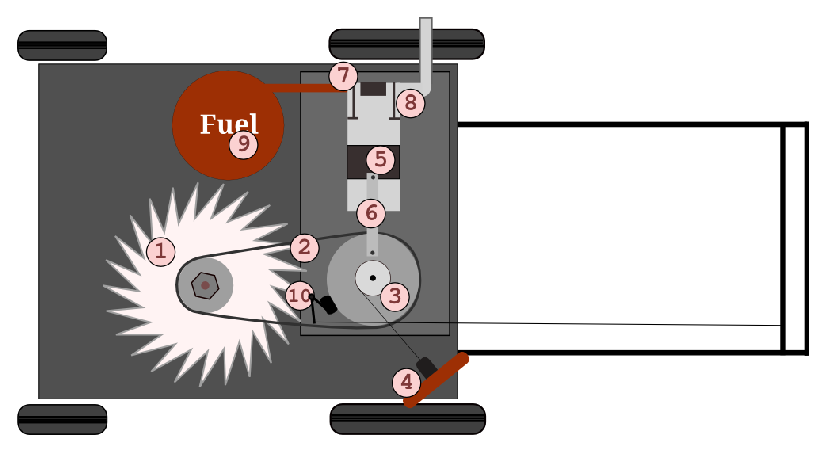
\includegraphics[scale= 0.8]{machine}
\caption{Proposed model of Lawn Mower}
\label{fig: image}
\end{center}
\end{figure}


\begin{figure}[ht!]
\centering
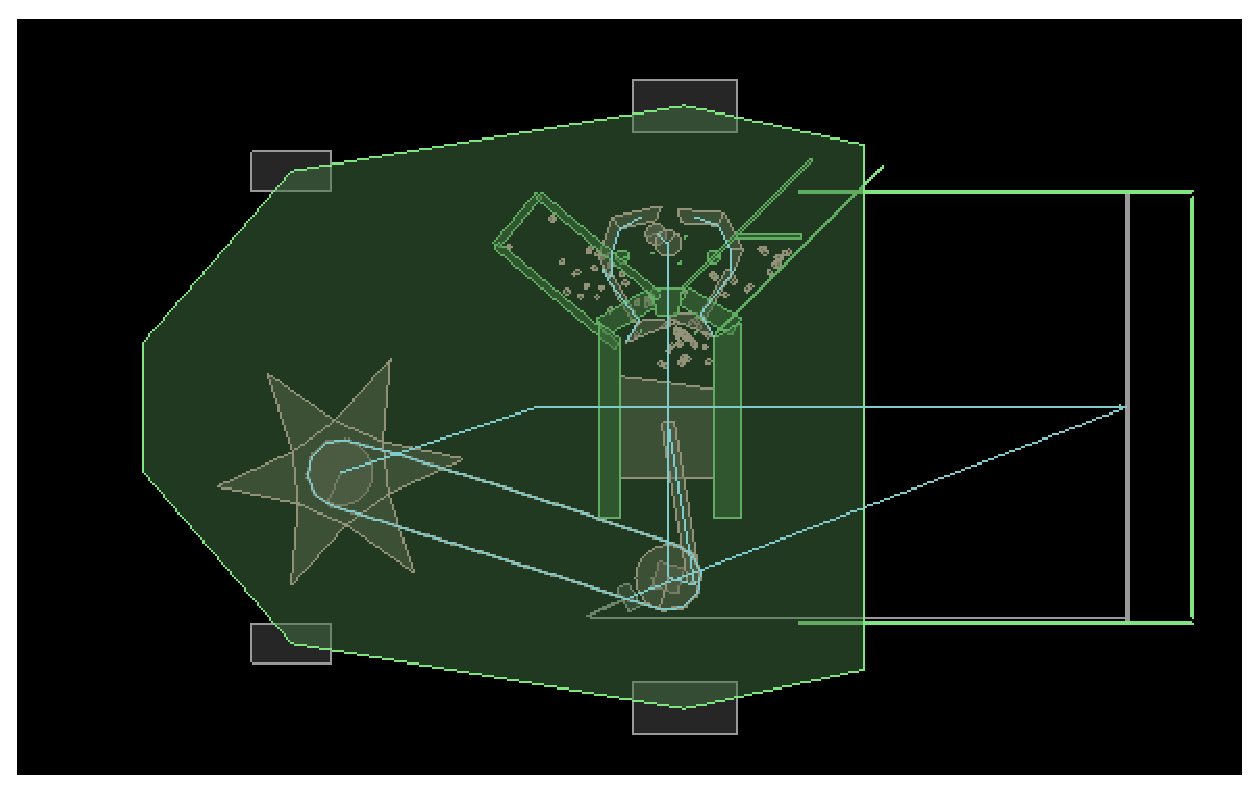
\includegraphics[scale=0.6]{lawnMower}
\caption{Implementation of Lawn Mower}
%\label{overflow}
\end{figure}

\pagebreak

\section*{USF of design}

\textbf{Automatically moving piston} \\
The whole assembly is not being driven by any external motor, the motion of piston is because of the simulated motion of fuel which will be triggered when the crank is given a initial torque by pressing the start button. 
\\ \linebreak
\textbf{Modelling of fluid} \\
Fluid is modelled as particles coming from the fuel chamber, when the fuel explodes the average velocity of the particles increases they gain high energy and try to escape out. 
\\ \linebreak
\textbf{Explosion of fluid particles} \\
 Explosion of fluid particles increases the average velocity, which is equivalent to conversion in state as the gaseous particles tends to have more velocity than in liquid phase. 
\cite{Sensor} 
 \\ \linebreak
\textbf{Ignition sensor} \\
The increase in velocity of the particles is controlled by a sensor, when this sensor is asserted the particles gains more velocity causing them to move faster. Sensors are also used to change the density of the particles to push the piston downwards. 
\cite{Sensor}
\\ \linebreak
\textbf{Auto fuel generation} \\
Fuel generation in the system is controlled by the speed at which fuel is being used up by the piston-assembly. If the rotor rotates faster means the blade has higher rpm them more fuel is generated. 
\\ \linebreak
\textbf{Keyboard Controls} \\
Machine can be stared using keyboard which gives an impulse to the rotor motor that sets everything in motion, Machine can be stopped by pull the rubber stopper which slows down the rotor motor and prevents creation of more fuel.
\\ \linebreak
\textbf{Smoke Filter}\\
Fuel is not directly thrown out of the system, it is allowed to pass through a filter ans coarse particles are destroyed in the system itself. Go Green!!
\pagebreak

\section*{Mechanism and Engine}
\subsection*{Piston Assembly}

Piston in the main engine is important for the ignition of fuel to keep the whole engine working, the basic principle behind working of fuel is :  \\
Fuel comes out of fuel chamber in liquid phase, because of high pressure exerted due to piston, fuel crosses its ignition point and gets converted to gas molecules. The gaseous molecule moves at higher speed in the piston chamber and pushes the piston downwards, the the process repeats causing the oscillatory motion of the piston. \\
The piston assembly also consist of the connector connecting piston to the rotating gear, the motion of piston causes the gear to rotate. \cite{piston} \\

\begin{figure}[ht!]
\centering
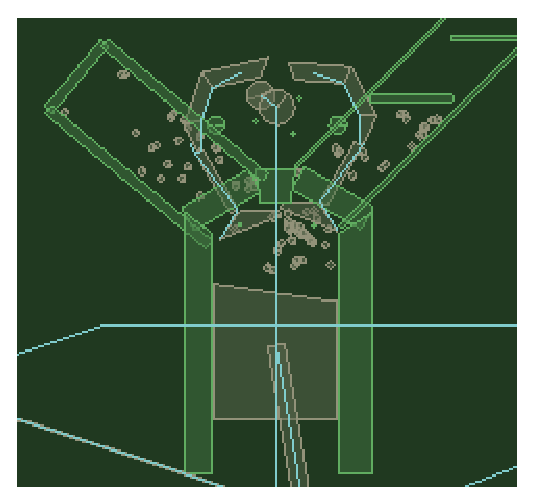
\includegraphics[scale=0.7]{pistonAssembly}
\caption{Piston Assembly}
%\label{overflow}
\end{figure}


\subsection*{Valve Assembly}

Valve in the simulation provide a passage for fuel to move from fuel chamber to piston  chamber periodically and when needed. Fuel tank generates fuel on its own(unlimitedly :D). This assembly also consist of a top-gear assembly that causes the to-and-fro motion of the valve, the right side of valve assembly has the smoke-outlet that provides way for the smoke to move out of the piston chamber. The two rods at the side along the two sides of the piston chamber prevents the fuel from moving out of the chamber.


\subsection*{Crank Shaft}

Central Rotor is the main connecting part that connects the piston-valve-assembly with the actual grass-cutting assembly. It is connected to blade through a conveyor belt, and to the piston with a solid connector. The motion of piston because of the fuel ignition causes the motion of this rotor, which then causes the gear in the blade to move because of friction, which further drives the main cutting blade. {CrankShaft}

\begin{figure}[ht!]
\centering
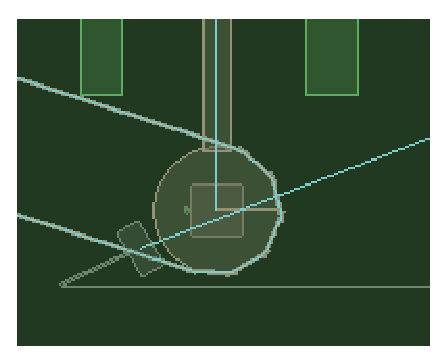
\includegraphics[scale=0.7]{crankShaft}
\caption{Crank Assembly}
%\label{overflow}
\end{figure}

\subsection*{Cutting Blade}

Cutting blade is indeed the actual cutting tool in the lawn mower driven by several gears connected to it as explained above. The Blade is connected to a central circular wheel that can rotate around its center, further the rotation of the wheel causes the rotation of the blade. The wheel is wrapped around by a conveyor belt as described above.

\begin{figure}[ht!]
\centering
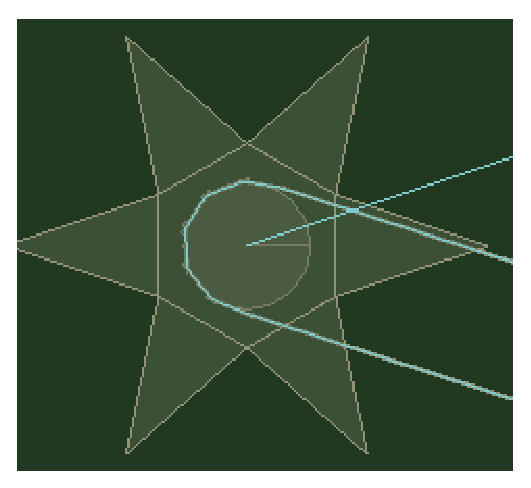
\includegraphics[scale=0.5]{bladeGear}
\caption{Blade Assembly}
%\label{overflow}
\end{figure}
\pagebreak

\section*{Profiling and Timing}
As most of the simulation revolves around bodies colliding with each other to generate events, we have optimized those function by manually tweaking the parameters position/velocity/number of particles etc. We have tried different values for optimised angles and the velocities and chosen the one that suits our need. In Debug mode maximum time is taken by findMaxSeperation function which is predefined in Box2D, we believe that the large time is because of the large number of collision that are taking place in our system; whereas in release mode the function that is taking maximum time is CollideEdgeandPoygon.
\cite{profile}
The call graph we got is flat as all the data values are quite low. \\ \linebreak
\textbf{Release Mode} \\ \linebreak
%\begin{figure}
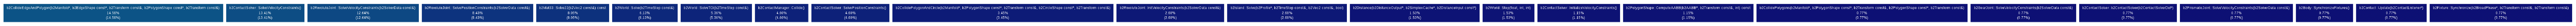
\includegraphics[scale=0.04]{release_mode} \\ \linebreak
%\caption{Call Graph:Release Mode}
%\label{overflow} \\ \linebreak
%\end{figure} 
\textbf{Debug Mode} \\ \linebreak
%\begin{figure}
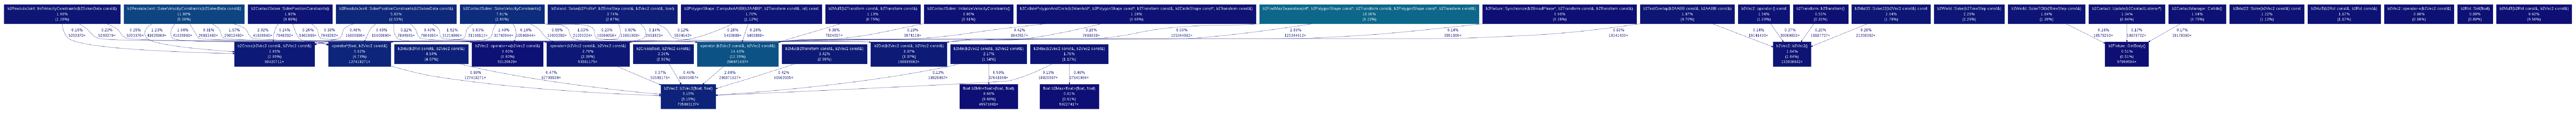
\includegraphics[scale=0.045]{debug_mode}
%\caption{Call Graph:Debug Mode}
%\label{overflow}
%\end{figure}


\section*{Interpolation of Graphs}
\par We plotted 5 graphs for analysing various parameters like Step-time, Loop-time. Below, we give a detailed description of those graphs.
\subsection*{Plot describing Average step and loop time (Y) over Iteration values (X)}
\par The plot in the following "figure-6" shows the relationship between the number of iterations and the average loop time as well as average step time.

The average step time for every iteration on X-axis varies as it is the time for one step which include all the background processes which consumes some constant time on that particular system. So, for more number of iterations, this time is divided and as a result, "average step time" decreases. 

The loop time is the total time for the 'for' loop to run with number equal to 'iteration number', and hence, it is obvious that loop-time will increase as we go forard in +x-direction.

\begin{figure}
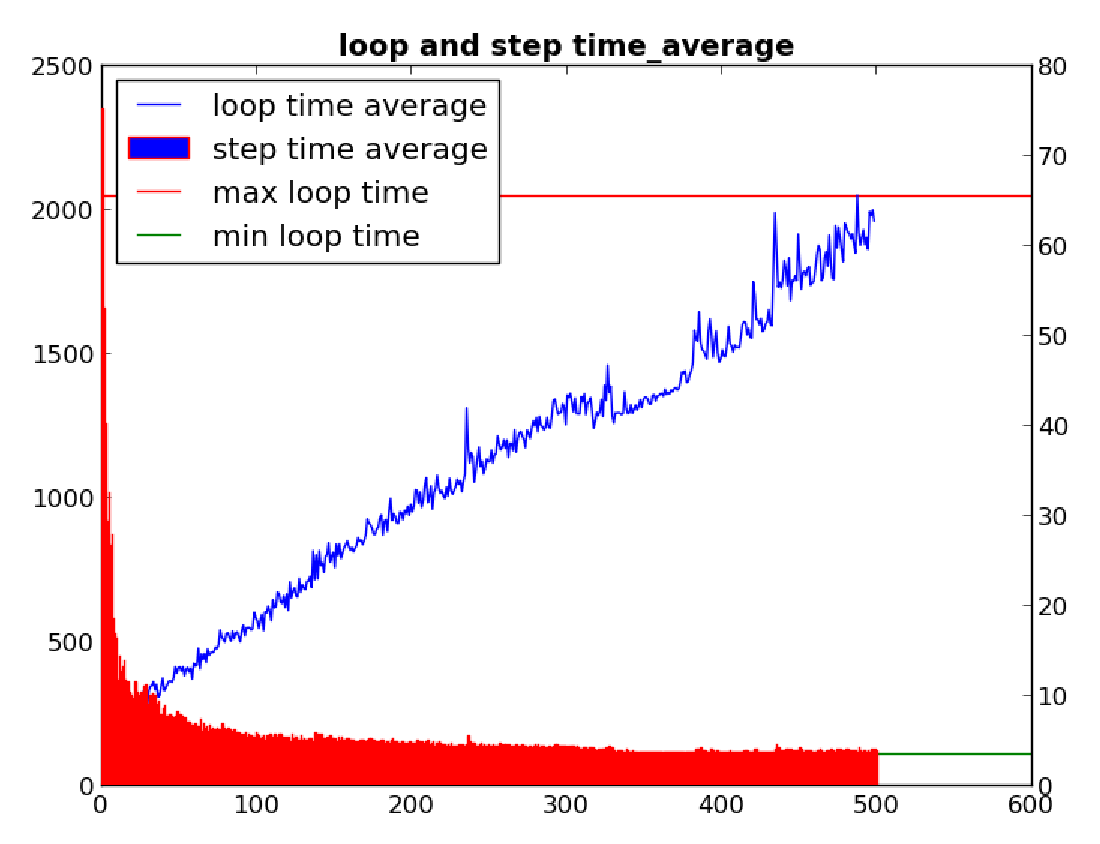
\includegraphics[width=12cm,height=8cm]{g20_project_plot01} 
\label{fig:plt1}
\caption{Average step time and loop time} 
\end{figure}

\subsection*{Plot descibing all the averages(Y) over Iteration number(X)}
\par The graph in figure-7 describes the average times for r velocity, position and collision. These plots follow the same reasoning as the average step-time over iterations in figure 1.

For a certain number of iterations, sum of position-update, velocity-update and collision update takes more time than their individual times and lesser than average seperation time. Moreover, velocity-updates takes more time than collision calculations which in turn takes slightly more time than position-update time. Because, the positions are first updated, which inturn is used to calculate the collisions, which updates the velocities of the bodies.

\begin{figure}
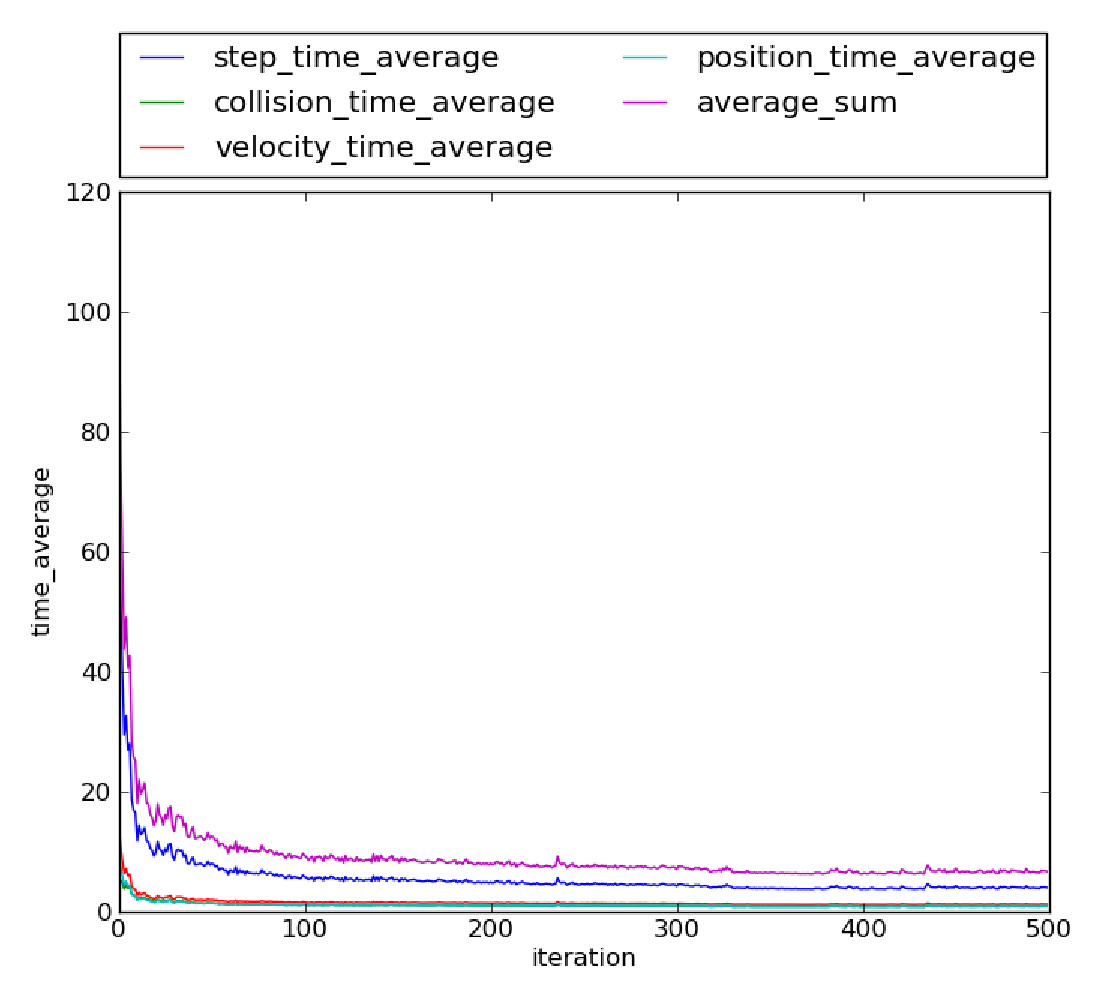
\includegraphics[width=12cm,height=8cm]{g20_project_plot02} 
\label{fig:plt2}
\caption{All the averages and updates over Iteration number} 
\end{figure}


\subsection*{Analysis of the Error bars of Avg step time over Iterations}
\par Variable-1(Number of Reruns) : We varied the number of reruns and created graphs. We noticed that, with lower number of reruns, the errorbars are low(close to the average). When the number of reruns are very high, the error bars are more elongated. Similar to, when the samples are higher in number, there would be a greater chance to have distant outliers.

Variable-2(Number of Iterations) : When the iteration number increases, the loop run for more time giving more possibility that step-time deviates from the mean. Hence, when the number of iterations is increasing towards '+ve X-axis', the average is damping towards '0' and the error bar is more deviated from the mean-point.


\begin{figure}
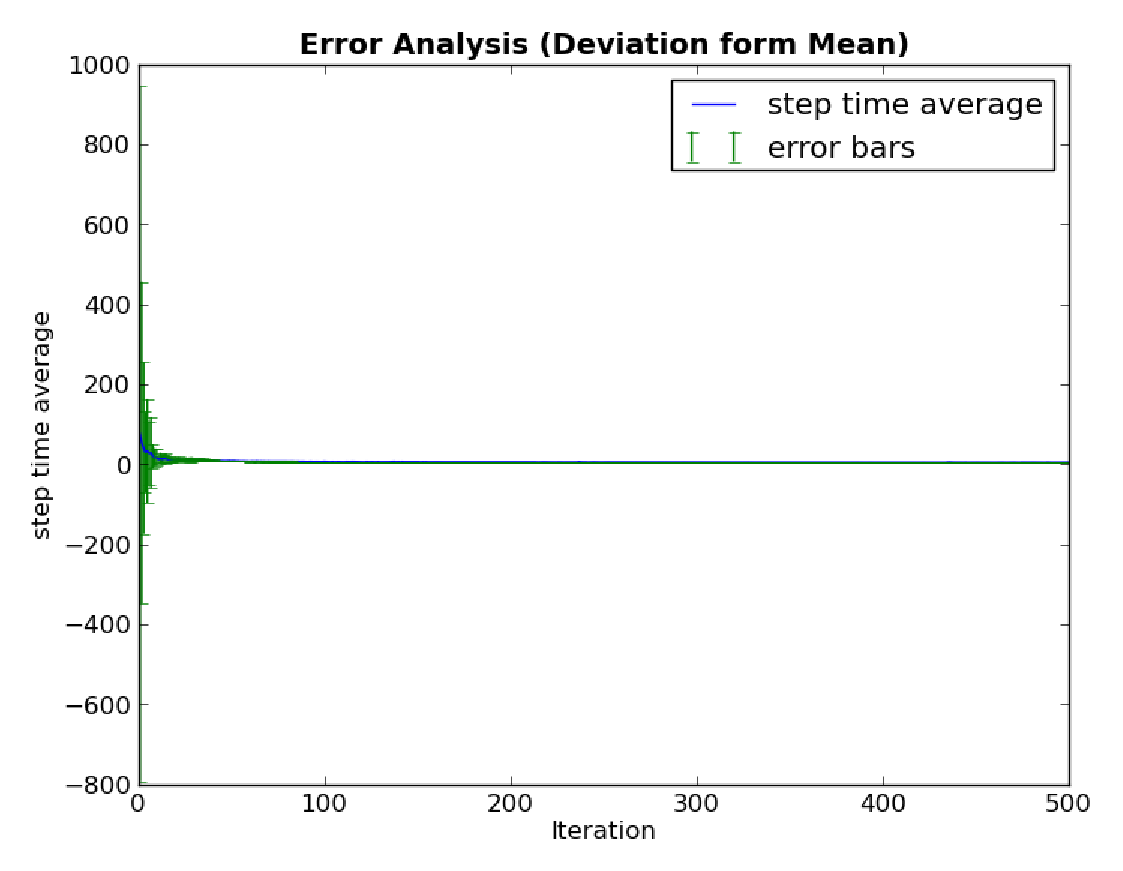
\includegraphics[width=12cm,height=8cm]{g20_project_plot03} 
\label{fig:plt3}
\caption{Analysis of the Error bars of Avg step time} 
\end{figure}



\subsection*{Analysis of Frequency plot of the step times and cumulative graph}
\par Most of the observations for average step times with different rerun numbers behave similarly, i.e., the height of the bars relatively will be proportional. They are nearly in the same area as suggested by the frequency histogram of figure-9 of average step time. If we decrease the length of partition on X-axis, the data would be more accurate. 

The slope of the cumulative graph will explain the possibility of the plot in that region on X-axis. The more the slope of the cumulative graph, the more is the probability of plot in that region.


\begin{figure}
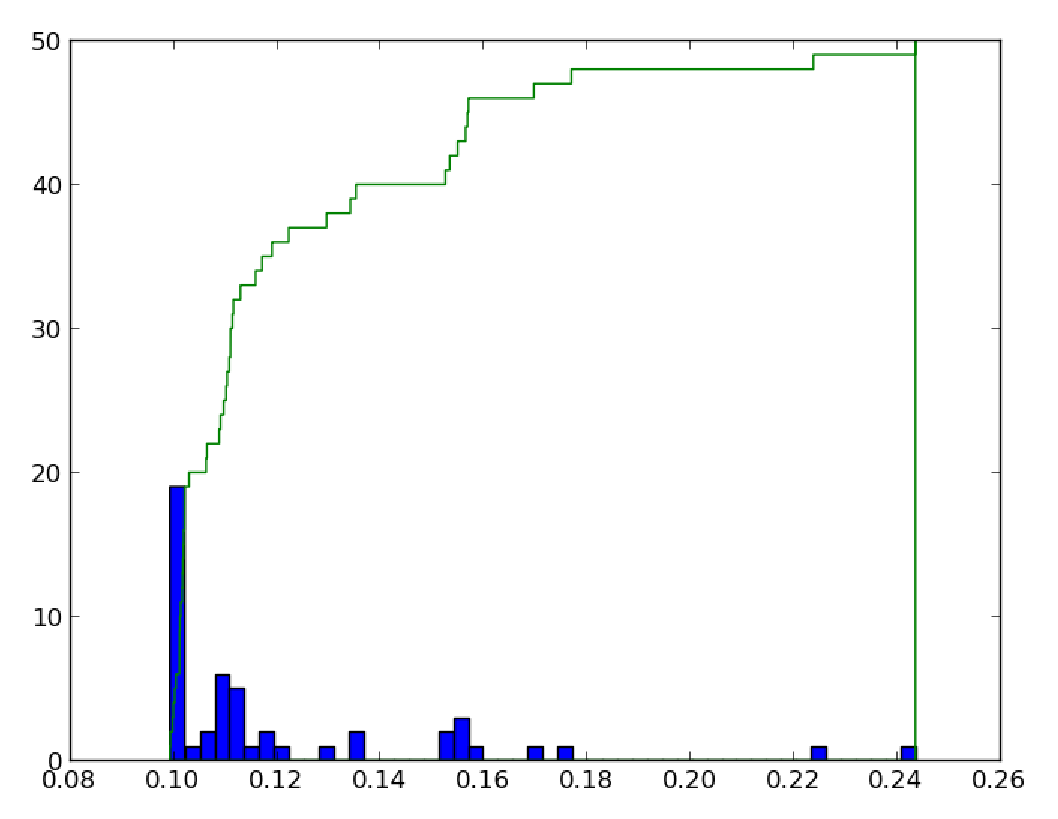
\includegraphics[width=12cm,height=8cm]{g20_project_plot04} 
\label{fig:plt4}
\caption{Frequency plot of the step times and cumulative graph} 
\end{figure}



\subsection*{Plot of Best Fit line for step time averaged}
\par There are two plots described in figure 10., one with average step time over all reruns and other with average step time over some random reruns.

As the number of iterations increase, the average step-time values are nearer to each other and the graphs start behaving similarly. As a result,for a particular iteration value, if we increase the number of iterations, the average distance between corresponding points on two graphs decreases and the best fit line seem to converge.

This is due to the fact that average for randomly executed reruns is more accurate for larger value of iterations.

We could see considerable difference in the best fit line when executed for smaller iterations. Also, increase number of reruns helps in converging both the best-fit lines.

\begin{figure}
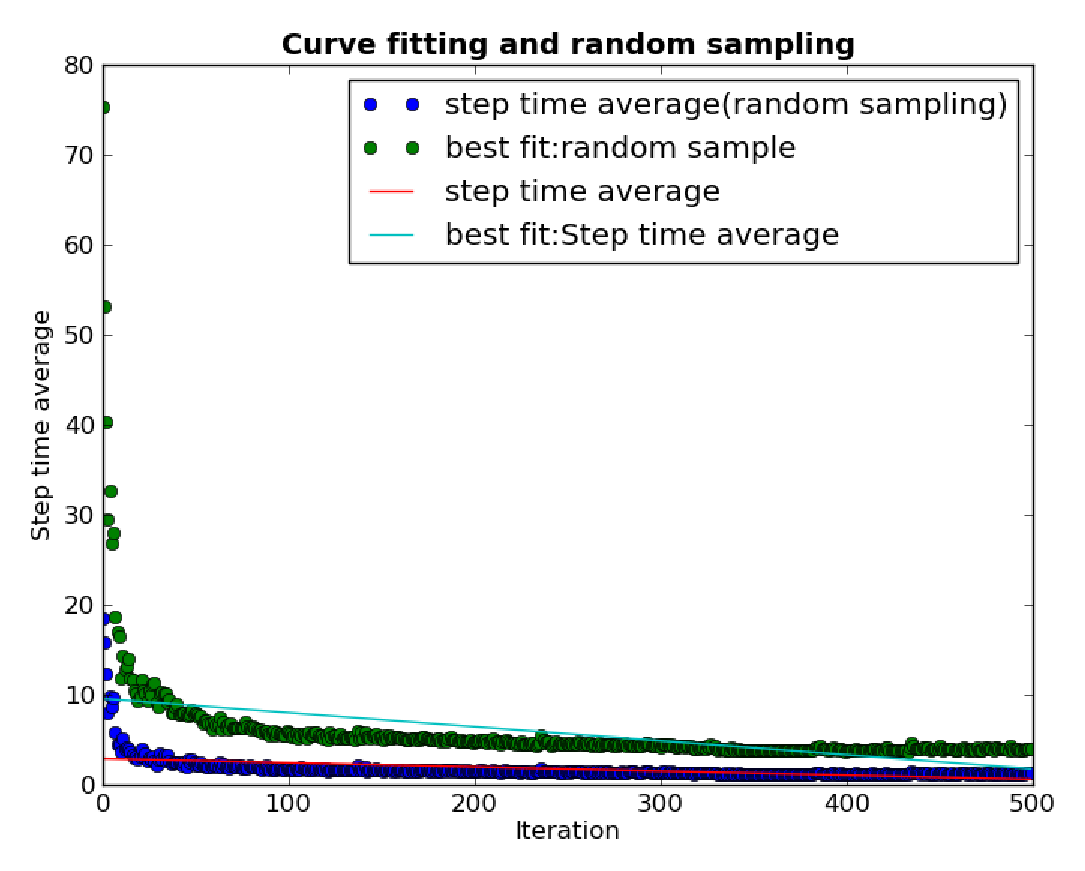
\includegraphics[width=12cm,height=8cm]{g20_project_plot05} 
\label{fig:plt5}
\caption{Best Fit line for step time averaged} 
\end{figure}

\pagebreak
\section*{Conclusion and Difference}
\paragraph{} The simulation gives an almost perfect approximation of the lawn mower machine and any 4-stroke engine under certain assumptions.
Box2d provides a good framework for physics simulation and is useful to demonstrate working of engine.

Difference from the design proposed earlier:
\begin{itemize}
\item Instead of making a starting wire, we have made a start button (Keyboard Input) to facilitate the working of lawn mower, and to keep the design cleaner.
\item Some new parts like the support valve on the two sides are added to make the design more robust.	\cite{Latex}
\end{itemize}

\bibliography{g20_project_report}
\bibliographystyle{unsrt}
\end{document}